\documentclass[a4paper]{article}

\usepackage[utf8]{inputenc}
\usepackage[portuguese]{babel}
\usepackage{indentfirst}
\usepackage{graphicx}
\usepackage{float}
\usepackage{fancyvrb}
\usepackage{color}
\newcommand*{\escape}[1]{\texttt{\textbackslash#1}}
\newcommand*{\escapeI}[1]{\texttt{\expandafter\string\csname #1\endcsname}}
\newcommand*{\escapeII}[1]{\texttt{\char`\\#1}}



\title{Projeto de Sistemas Operativos\\\textit{Stream Processing}}
\author{Mariana Miranda (a77782) \and Daniel Fernandes {a78377}\and Helena Poleri (a78633)}
\begin{document}
\maketitle
\pagebreak

\section{Introdução}

Neste trabalho pretendeu-se construir um sistema de \textit{stream processing}. Estes sistemas utilizam uma rede de componentes para filtrar, modificar e processar um fluxo de eventos. Tipicamente, permitem tratar uma grande quantidade de dados explorando a concorrência tanto entre etapas sucessivas (\textit{pipelining}) como entre instâncias do mesmo componente. Um exemplo de um sistema de \textit{stream processing} para
sistemas distribuídos é o \textit{Apache Storm}.

Neste caso, pretendeu-se uma implementação para sistemas Unix, explorando a semelhança de \textit{stream processing} com os filtros de texto compostos em pipeline. Sendo assim, assume-se que cada evento é uma linha de texto, com campos separados por dois pontos (:), sendo o seu tamanho inferior a PIPE BUF.

Este trabalho tem duas partes: a implementação de um conjunto de componentes, que realizam tarefas elementares; e a implementação do sistema que compõe e controla a rede de processamento.

\section{Concepção da Solução}

\subsection{Componentes}

Uma função que usamos para nos auxiliar em todos os problemas desta primeira parte (e do Controlador também), foi uma \textit{readln}. Esta função lê uma linha de um descritor de ficheiro, com o auxílio da \textit{system call} read. Esta última lê do descritor um certo número de \textit{bytes} e coloca-os num \textit{buffer}.

Nesta versão, estamos a ler mais do que um carater de cada vez (neste caso, o tamanho do PIPE BUF), para reduzir o número de \textit{system calls}. Por consequência, isto reduz também o tempo de execução.

\begin{Verbatim}[obeytabs]
int readln(char* buf, int* r, int* pos, char* line) {
	int i;
	if (*pos == 0) *r = read(0, buf, PIPE_BUF);
	for (i = 0; buf[*pos] != '\n'; (*pos)++, i++) {
		if (*pos == *r) {
			*r = read(0, buf, PIPE_BUF);
			*pos = 0;
		}
		line[i] = buf[*pos];
	}
	if ((*r) == -1) {
		perror("Erro na leitura!");
		_exit(-1);
	}
	(*pos)++;
	line[i++] = '\n';
	line[i] = '\0';
	return ((*r) == 0) ? 0 : i;
}
\end{Verbatim}

Outra função da qual necessitamos para a maioria dos problemas foi a função \textit{split} que se segue.

\begin{Verbatim}[obeytabs]
void split(char* str, char** res, int n) {
	int i, j = 0;
	res[j++] = str;
	for (i = 0; str[i]; i++) {
		if (str[i] == ':') {
			str[i] = '\0';
			if (j == n) res = realloc(res,
			  (n + 5) * sizeof (char*));
			res[j++] = &(str[i + 1]);
		}
	}
}
\end{Verbatim}

Usamos porque, tendo que fazer operações sobre as diferentes colunas do \textit{input}, às vezes necessitamos de saber o valor de cada uma destas. Então o que esta função faz é dividir os argumentos passados em diferentes \textit{strings}, colocando estas em \textit{res}, uma lista destas \textit{strings}.

\subsubsection{const \textless valor\textgreater}

Este programa reproduz no \textit{stdout} as linhas recebidas no seu \textit{stdin} acrescentando uma nova coluna sempre com o mesmo valor.

\begin{Verbatim}[obeytabs]
void _const(char* arg) {
	int nr, r, n = strlen(arg) + 2, pos = 0;
	char buf[PIPE_BUF], line[PIPE_BUF + n];
		while ((nr = readln(buf, &r, &pos, line)) != 0) {
		line[nr - 1] = '\0';
		nr = sprintf(line, "%s:%s\n", line, arg);
		write(1, line, nr);
	}
}
\end{Verbatim}

Enquanto não for pressionado Ctrl+D, vão ser sempre lidas as linhas do \textit{stdin}, uma a uma. Depois de lida uma linha, esta é processada e formatada com a função \textit{sprintf}, que lhe acrescenta a coluna com o valor passado como parâmetro. É essa linha formatada que é escrita no \textit{stdout}.

\subsubsection{filter \textless coluna\textgreater \textless operador\textgreater \textless operando\textgreater}

Este programa reproduz no \textit{stdout} as linhas que satisfazem uma condição indicada nos seus argumentos.

Como tínhamos várias condições diferentes para tratar (se é diferente, se é maior, etc.), temos uma função que verifica qual das condições é recebida e que, dependendo disso, invoca a função seguinte com a função adequada passada como parâmetro.

\begin{Verbatim}[obeytabs]
void _filterS(int col1, int col2, int (*f)(int, int)) {
	int nr, r, pos = 0;
	char buf[PIPE_BUF], line[PIPE_BUF], linecp[PIPE_BUF];
	char** res = (char**) malloc (10 * sizeof (char*));
	while((nr = readln(buf, &r, &pos, line)) != 0) {
		strcpy(linecp, line);
		linecp[nr - 1] = '\0';
		split(linecp, res, 10);
		if(f(atoi(res[col1]), atoi (res[col2])))
			write(1, line, nr);
	}
}
\end{Verbatim}

Aqui, enquanto não for pressionado Ctrl+D, vão ser sempre lidas as linhas do \textit{stdin}, uma a uma. Depois de lida uma linha, usa-se a split para podermos saber os valores das colunas pretendidas. A partir daí, é necessário apenas verificar, usando a função passada como parâmetro, se a condição passada como argumento é verdadeira. Se for, escreve-se no \textit{stdout}.

\subsubsection{window \textless coluna\textgreater \textless operação\textgreater \textless linhas\textgreater}

Este programa reproduz todas as linhas acrescentando-lhes uma nova coluna com o resultado de uma operação calculada sobre os valores da coluna indicada nos argumentos para as N linhas anteriores (sendo N o último argumento).

À semelhança do que aconteceu com a \textit{filter}, tínhamos que lidar com várias operações diferentes (soma, média, etc). Então, também aqui temos uma função que verifica qual das operações é recebida e que, dependendo disso, invoca a função seguinte com a função adequada passada como parâmetro.

\begin{Verbatim}[obeytabs]
void _add (int col, int nval, int (*f)(int*, int)) {
	ArrayC array = criaArrayC(nval);
	int nr, r, pos = 0;
	char buf[PIPE_BUF], line[PIPE_BUF], linecp[PIPE_BUF];
	char** res = (char**) malloc (10 * sizeof (char*));
	while ((nr = readln(buf, &r, &pos, line)) != 0) {
		line[nr - 1] = '\0';
		strcpy(linecp, line);
		split(linecp, res, 10);
		nr = sprintf(line, "%s:%d\n", line,
		   f(array -> values, array -> nVals));
		addArrayC(array, atoi(res[col]));
		write(1, line, nr);
	}
}
\end{Verbatim}

Para nos ajudar na implementação desta função, criamos uma estrutura de \textit{array} circular, para guardar lá apenas os valores que nos interessam das linhas anteriores (imaginando que temos que ter em conta as 3 linhas anteriores, apenas estarão lá sempre os valores das 3 linhas imediatamente anteriores à atual).

Depois de ter isso, é apenas necessário ler as linhas do \textit{stdin}, uma a uma, dividi-las usando a split para que se possa guardar apenas o valor necessário no array circular, e formatar a linha (usando a \textit{sprintf}) de modo a acrescentar uma nova coluna com o resultado de aplicar a função passada como argumento aos valores do array circular.

De seguida, escreve-se essa linha formatada no \textit{stdout}.

\subsubsection{spawn \textless cmd\textgreater \textless args...\textgreater}

Este programa reproduz no \textit{stdout} todas as linhas recebidas no \textit{stdin}, executando o comando recebido como argumento uma vez para cada uma delas, e acrescentando uma nova coluna com o respectivo \textit{exit status}.

\begin{Verbatim}[obeytabs]
void _spawn (int argc, char** argv) {
	char* arg;
	int status, i, nr, r, pos = 0;
	char buf[PIPE_BUF], line[PIPE_BUF], linecp[PIPE_BUF];
	char** argvcp = (char**) malloc((argc + 1) * sizeof (char*));
	char** res = (char**) malloc (10 * sizeof (char*));
	argvcp[argc] = NULL;
	while ((nr = readln(buf, &r, &pos, line)) != 0) {
		line[nr - 1] = '\0';
		strcpy(linecp, line);
		split(linecp, res, 10);
		for (i = 0; i < argc; i++) {
			if (argv[i][0] == '$') 
			   argvcp[i] = res[atoi(&(argv[i][1])) - 1];
			else argvcp[i] = argv[i];
		}
		if (!fork()) {
			execvp(argvcp[0], argvcp);
			_exit(-1);
		} else {
			wait(&status);
			status = WEXITSTATUS(status);
		}
		nr = sprintf(line, "%s:%d\n", line, status);
		write(1, line, nr);
	}
}
\end{Verbatim}

Esta função lê as linhas do \textit{stdin}, uma a uma, divide-as usando a \textit{split} e prossegue a substituir os argumentos que começam com um \$ pelo o que está na coluna indicada. De seguida, cria um \textit{fork()} e o filho do processo vai executar o comando. De seguida, a linha recebida é formatada e é-lhe adicionada uma linha contendo o \textit{exit status}, usando a função \textit{sprintf}. Esta linha formatada é escrita no \textit{stdout}.

\subsection{Controlador}

O primeiro passo para resolver o problema do controlador, foi planear a sua solução. A ideia geral pode ser ilustrada através do seguinte esquema:

\begin{figure}[H]
	\centering
	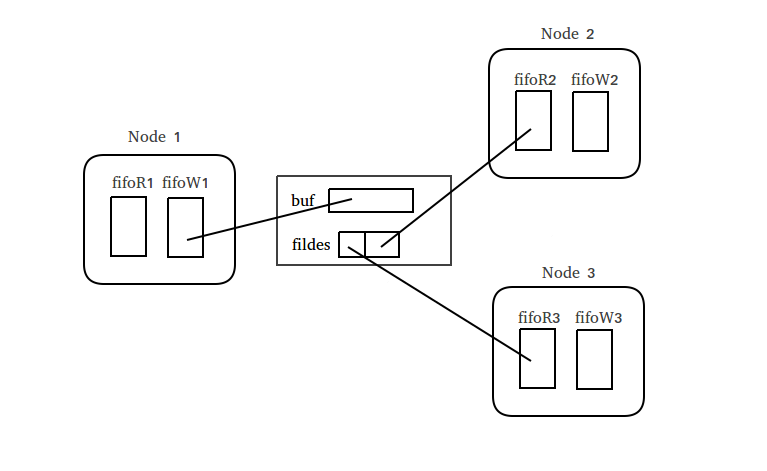
\includegraphics[width=\textwidth]{esquema.png}
	\caption{Ideia geral do trabalho}
	\label{fig:esquema}
\end{figure}

\subsubsection{Node}

Como podemos ver, a ideia era ter um conjunto de nodos, cada um constituído por dois FIFOs, um destinado à leitura e outro destinado à escrita, e pelo PID de um processo com os redireccionamentos correspondentes.

Os FIFOs estão nomeados de acordo com o seu ID e tipo (leitura (R) ou escrita (W)) no seguinte formato:

\textbf{pipe\textless R/W\textgreater\textless ID\textgreater}

\subsubsection{Connect}

As conexões estão a ser feitas por intermédio de um processo, que tem o seu \textit{stdin} redireccionado para o fifo de escrita do nodo conector. Através deste redirecionamento e com o auxílio da \textit{readln}, as informações são transferidas para um \textit{buffer} interno ao processo. Tem ainda um \textit{array} onde ficam armazenados todos os \textit{file descriptors} dos fifos de leitura dos nodos aos quais conectar.

A função do processo em questão é, então, apenas ler do \textit{buffer} e escrever para cada um desses \textit{file descriptors}, efetuando assim as conexões.

\subsubsection{Estruturação das conexões}

As várias conexões encontram-se organizadas numa matriz, onde as linhas correspondem aos nodos de origem e as colunas aos nodos de destino. Imaginando que existem nodos de 1 a 7, adicionados por ordem, e que o nodo 1 está conectado aos nodos 6 e 7, então nas posições (1,6) e (1,7) vai estar armazenado o PID da conexão.

Na nossa implementação, é permitido que estes identificadores nos nodos, sejam passados por qualquer ordem e número, sendo que, ainda assim, na matriz, os nodos são colocados por ordem na mesma. Para isso, aliado à matriz, encontra-se um array que faz a conversão entre identificadores e posições na matriz (imaginando que o primeiro nodo dado tem o identificador 516, na matriz esse passará a corresponder a 1).

O porquê da criação deste \textit{array} será explicado mais adiante.

\subsubsection{Disconnect}

Uma vez que cada conexão liga um nodo origem para mais do que um destino, e de forma a preservar as restantes conexões, a única maneira de fazer o \textit{disconnect} era matar o processo que faz essa conexão e criar um novo para substitui-lo, com as implicações que isso acarreta (alterações na matriz, etc).

Matar um processo é tão fácil quanto procurar o seu PID na matriz.

\subsubsection{Inject}

A \textit{inject} cria um novo processo com o comando que lhe é passado como argumento, com os redireccionamentos certos, isto é, redireccionamento de output para o fifo de leitura do nodo (passado também como argumento). 

\subsubsection{Alteração de Componentes}

Na alteração de componentes, fizemos com que esta acontecesse caso fosse recebido um comando com o seguinte formato

\textbf{change\textless ID\textgreater\textless cmd\textgreater\textless args...\textgreater}

A solução passa por criar um novo processo com os mesmos redirecionamentos do já existente, alterando o PID do processo dentro do nodo correspondente e matando o anterior.

\subsubsection{Remoção de Nós}

A remoção de nodos foi provavelmente a parte mais complicada do projeto, pois não é tão simples quanto parece à primeira vista. O que acontece é que, imaginemos que temos as conexões seguintes (cada nodo representado como um círculo, a vermelho o nodo que queremos remover):

\begin{figure}[H]
	\centering
	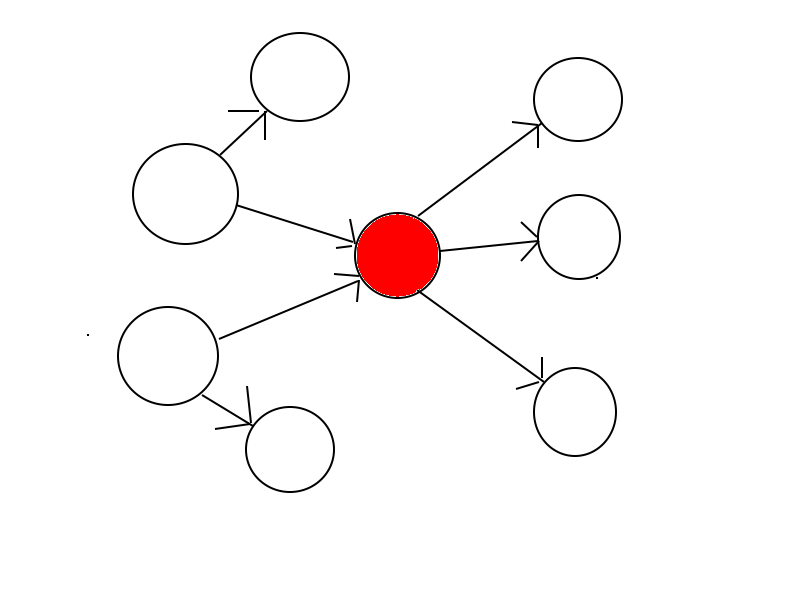
\includegraphics[width=\textwidth]{remove.png}
	\caption{Exemplo de conexões}
	\label{fig:remove}
\end{figure}

A situação de remover o nodo em questão, implica grandes alterações nas conexões em que ele está envolvido. Para remover os nodos que o têm como origem, é relativamente fácil: é apenas necessário procurar na matriz a linha correspondente ao nodo, e matar o PID existente na linha.

No entanto, quanto aos nodos que o têm como destino (nodos do lado esquerdo na figura), já não é tão simples, sendo necessário refazer todas as conexões. Isto acontece pois estas conexões, tem outros destinos e o mesmo processo. Para todos estes nodos que tem o nodo vermelho como destino, é necessário então refazer as conexões, alterando os PIDs na matriz de acordo.

Depois disto feito, resta na matriz eliminar a linha e coluna associada ao nodo removido. É aqui que entra a necessidade de possuir um \textit{array} que associa os identificadores dos nodos à posição correspondente na matriz, pois precisamos de remover a linha e coluna correspondente ao identificador do nodo.

\section{Conclusão}


O sistema de \textit{stream processing} criado, permite que os nós da rede, depois de criados, continuem a existir até serem removidos. O servidor vai recebendo comandos, devendo atuar perante cada um, atualizando a rede (acrescentando nós ou conexões), sendo estes comandos recebidos um por linha ou então especificados num ficheiro de configuração. As conexões podem ser adicionadas depois de os nós terem sido criados. A rede não para em momento nenhum, sendo que os erros são escritos para um ficheiro \textit{log}, e os comandos errados são ignorados.

Perante isto, pensamos que os objetivos pretendidos, de acordo com o enunciado, foram bem atingindos.


\end{document}